\section{Conjugated segments and rigid fragments}

Conjugated segments are described in a separate \xml file. An example for \dcvt is shown in listing~\ref{list:conjugated_segments}.


{\small 
\begin{tabular}{p{3cm} p{10cm}}
\xml tag & Description \\
\hline
 \texttt{posname} & Location of \xyz. \\
 \texttt{orbname} & Location of \orb. \\
 \texttt{basisset} & This should be set to INDO, unless the fort.7 has been created using another basis set. In that case it must be set to an \xml file setting the characteristics of the basis set. \\
 \texttt{transorb} & Number of HOMO (LUMO) orbital. Corresponds to the number of $\alpha$ electrons in the \gaussian log-file {get\_orbitals.log} minus one (since counting in C++ starts at zero) for the HOMO and the number of $\alpha$ electrons for the LUMO. \\
 \texttt{reorg} & Reorganization energy of the cation or anion in eV. \\
 \texttt{name} & Name of the mapping of the molecule. Must correspond to CG mapping.\\
 \texttt{energy} & Site energy of the conjugated segment. \\
 \texttt{monomer\_atom\_map} &
 List of atom indices as they were specified in the \gaussian input used to create the \orb file. 
 Note: The first three values are important, since they must correspond to the first three atoms defined in the coarse-grained mapping, which are used to calculate two vectors indicating the orientation of the molecule. The third required vector is the eigenvector of the smallest eigenvalue of the gyration tensor, i.e. perpendicular to the planar core.
 Note: The number of molecules here may differ from that in the coarse-grained mapping, since for example only the core is important for transport and not the side chains, but it has to be the same number of atoms as in the \gaussian input file otherwise overlap integral values will be terribly wrong. 
\end{tabular}



\clearpage
\begin{figure}[ht]
\centering
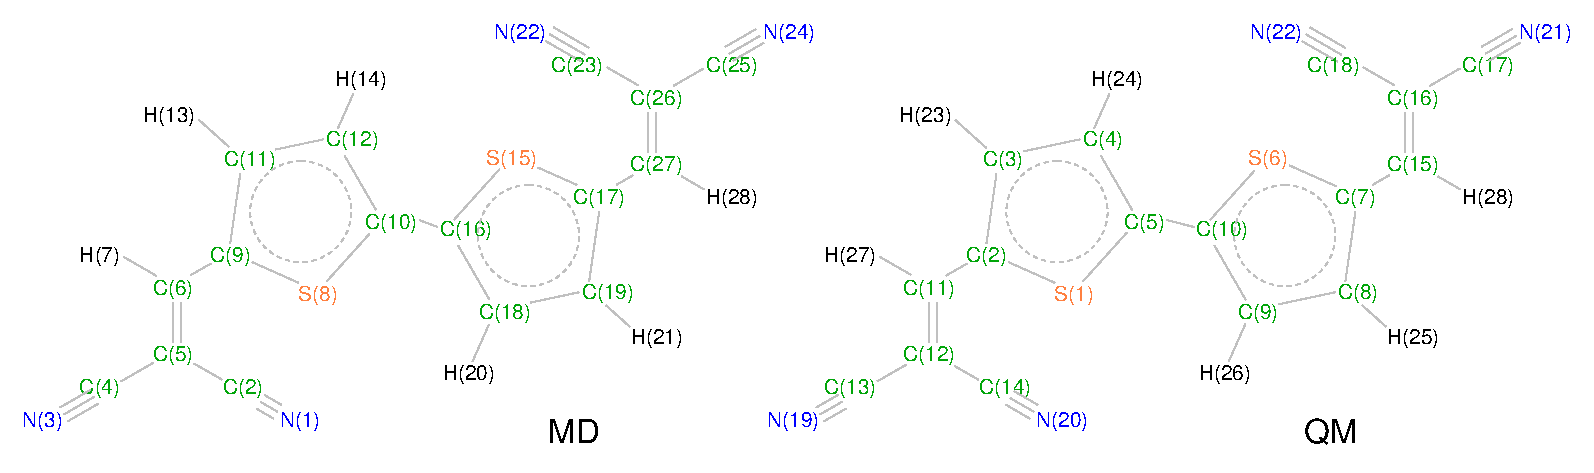
\includegraphics[width=\textwidth]{./fig/chemical_structure/dcv2t_gaussian} 
\caption{\small Atom order of \dcvt in the atomistic topology (MD) and qunatum chemical calculations (QM). The  link between two is established in the description of a conjugated segment shown in listing~\ref{list:conjugated_segments}.}
\label{fig:dcv2t_qm}
\end{figure}

\lstset{
  language=XML,
  frame=lines,
  basicstyle=\ttfamily\footnotesize,
  identifierstyle=\color{red},
  keywordstyle=\color{blue},
  showstringspaces=false,
  columns=fullflexible,
  commentstyle=\color{gray}\rmfamily\itshape,
  morekeywords={crgunit_type,ChargeUnitType,posname,orbname,basisset,transorb,reorg,nameneutr,namecrg,energy,beadconj,molname,name,monomer_atom_map,monomer_atom_weights},
}

\lstinputlisting[
 label=list:conjugated_segments, 
 caption={\small \xml file describing conjugated segments.
}]%
{./input/segments.xml}
\clearpage

%\noindent
%\suggestion{%
%crgunit\_type -> ConjugatedSegmentTypes \\ 
%ChargeUnitType -> ConjugatedSegmentType \\ 
%posname -> CoordinatesFile \\
%orbname -> OrbitalsFile \\
%transorb -> TransportOrbital \\
%reorg -> ReorganizationEnergy (do we need this here?) \\
%nameneutr -> ChargesNeutralFile \\
%namecrg -> ChargesChargedFile (do we need this here?) 
%}


